\section{conversion.c File Reference}
\label{conversion_8c}\index{conversion.c@{conversion.c}}
{\tt \#include $<$stdio.h$>$}\par
{\tt \#include \char`\"{}conversion.h\char`\"{}}\par
{\tt \#include \char`\"{}vi\_\-table.h\char`\"{}}\par
{\tt \#include \char`\"{}ueac.h\char`\"{}}\par
{\tt \#include \char`\"{}filter.h\char`\"{}}\par
{\tt \#include \char`\"{}global.h\char`\"{}}\par


Include dependency graph for conversion.c:\begin{figure}[H]
\begin{center}
\leavevmode
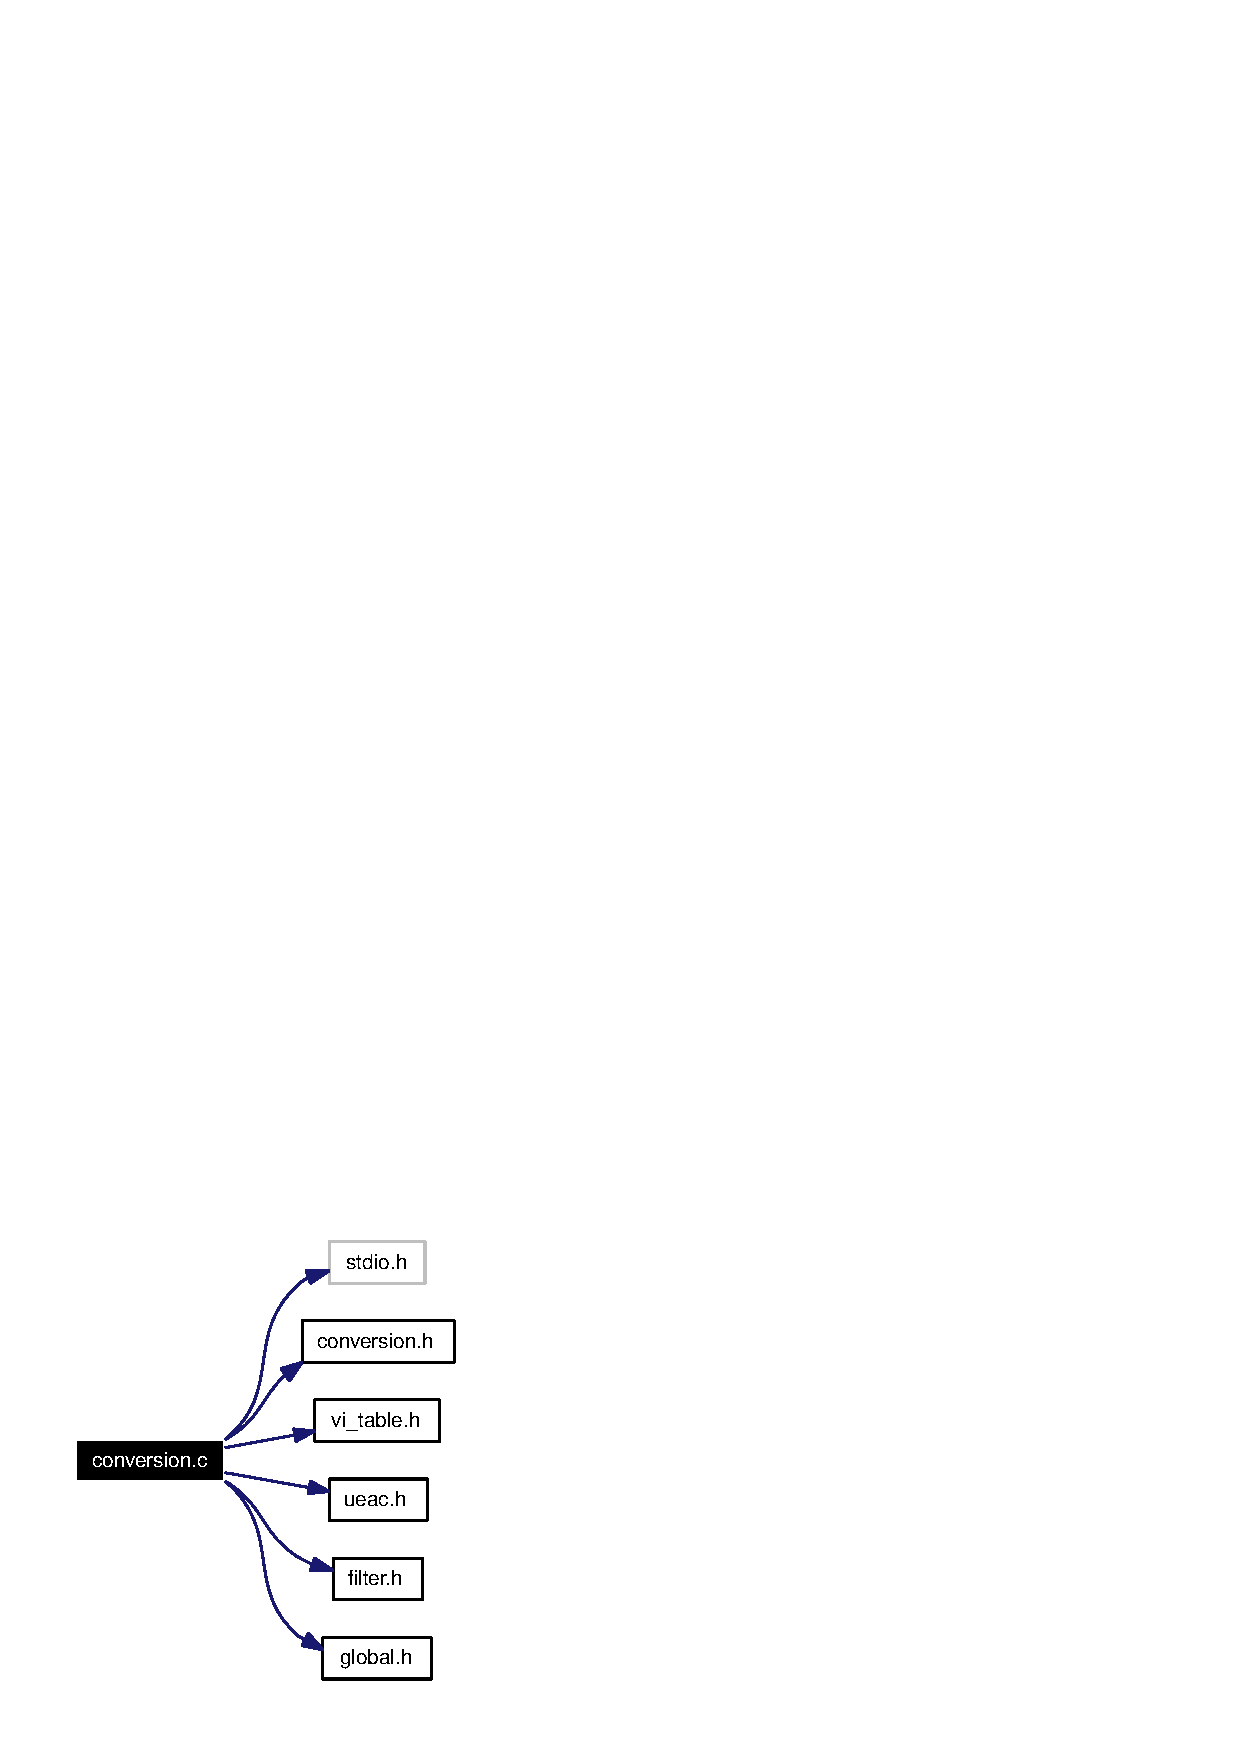
\includegraphics[width=109pt]{conversion_8c__incl}
\end{center}
\end{figure}
\subsection*{Functions}
\begin{CompactItemize}
\item 
void {\bf convert\_\-a2d} (char value\_\-type, unsigned short a2d\_\-data, {\bf ueacval\_\-t} $\ast$return\_\-val, int pin)
\end{CompactItemize}


\subsection{Function Documentation}
\index{conversion.c@{conversion.c}!convert_a2d@{convert\_\-a2d}}
\index{convert_a2d@{convert\_\-a2d}!conversion.c@{conversion.c}}
\subsubsection{\setlength{\rightskip}{0pt plus 5cm}void convert\_\-a2d (char {\em value\_\-type}, unsigned short {\em a2d\_\-data}, {\bf ueacval\_\-t} $\ast$ {\em return\_\-val}, int {\em pin})}\label{conversion_8c_a0}




Definition at line 61 of file conversion.c.

References a2d\_\-i\_\-conversion, ueacval::hundredth, cal::i\_\-in\_\-floor, cal::i\_\-in\_\-offset, ueacval::integer, ueac::pin\_\-cal, ueac\_\-state, and V\_\-CONVERSION.

Referenced by current\_\-output\_\-calibration(), evaluate\_\-lla(), print\_\-grid\_\-i(), print\_\-grid\_\-v(), scan\_\-probes(), and ueac\_\-execute\_\-instruction().

\footnotesize\begin{verbatim}61                                                                                         {
62   if (value_type==V_CONVERSION) {
63     if (a2d_data < 400) {
64       return_val->integer=0;
65       return_val->hundredth=a2d_data>>2;
66     }
67     else if (a2d_data < 800) {
68       return_val->integer=1;
69       return_val->hundredth=(a2d_data-400)>>2;
70     }
71     else if (a2d_data < 1200) {
72       return_val->integer=2;
73       return_val->hundredth=(a2d_data-800)>>2;
74     }
75     else if (a2d_data < 1600) {
76       return_val->integer=3;
77       return_val->hundredth=(a2d_data-1200)>>2;
78     }
79     else if (a2d_data < 2000) {
80       return_val->integer=4;
81       return_val->hundredth=(a2d_data-1600)>>2;
82     }
83     else if (a2d_data < 2400) {
84       return_val->integer=5;
85       return_val->hundredth=(a2d_data-2000)>>2;
86     }
87     else if (a2d_data < 2800) {
88       return_val->integer=6;
89       return_val->hundredth=(a2d_data-2400)>>2;
90     }
91     else if (a2d_data < 3200) {
92       return_val->integer=7;
93       return_val->hundredth=(a2d_data-2800)>>2;
94     }
95     else if (a2d_data < 3600) {
96       return_val->integer=8;
97       return_val->hundredth=(a2d_data-3200)>>2;
98     }
99     else if (a2d_data < 4000) {
100       return_val->integer=9;
101       return_val->hundredth=(a2d_data-3600)>>2;
102     }
103     else {
104       return_val->integer=10;
105       return_val->hundredth=(a2d_data-4000)>>2;
106     }
107   }
108   else {
109     return_val->integer=a2d_i_conversion[a2d_data];
110     if (pin<25) {
111       if (return_val->integer<=ueac_state.pin_cal[pin].i_in_floor) {
112         return_val->integer=0;
113       }
114       else {
115         return_val->integer+=ueac_state.pin_cal[pin].i_in_offset;
116       }
117     }
118     return_val->hundredth=0;
119   }
120 }
\end{verbatim}\normalsize 


